% Problem 4/6 solution
\noindent
\underline{Solution:}\\

\noindent
The orbitals $S_1$ and $S_2$ can be visualized as shown below (the first figure).
\begin{figure}[h]
\centering
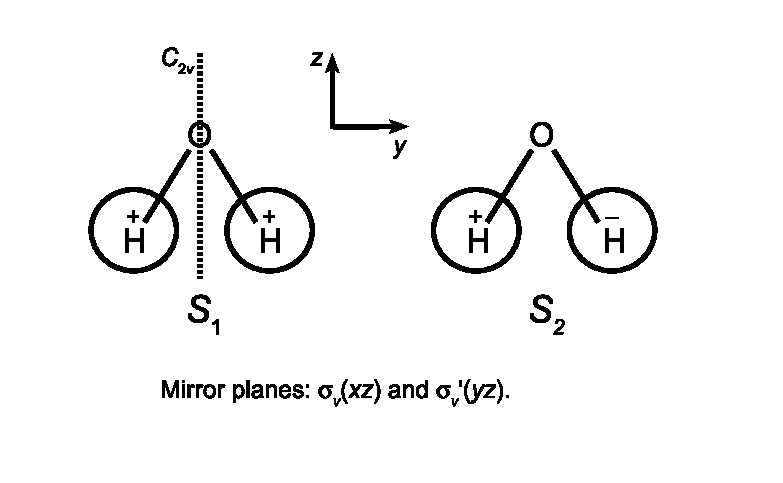
\includegraphics[scale=0.45]{watermo}
\caption{Visualization of $S_1$ and $S_2$ orbitals.}
\end{figure}
From this we can see that $S_1$ corresponds to $A_1$ (all operations give 1) and $S_2$ to $B_2$ (characters 1 $-1$ $-1$ 1).
The symmetry labels for the orbitals are therefore $a_1$ and $b_2$, respectively. The oxygen atom orbitals are shown in the second figure below.
\begin{figure}[h]
\centering
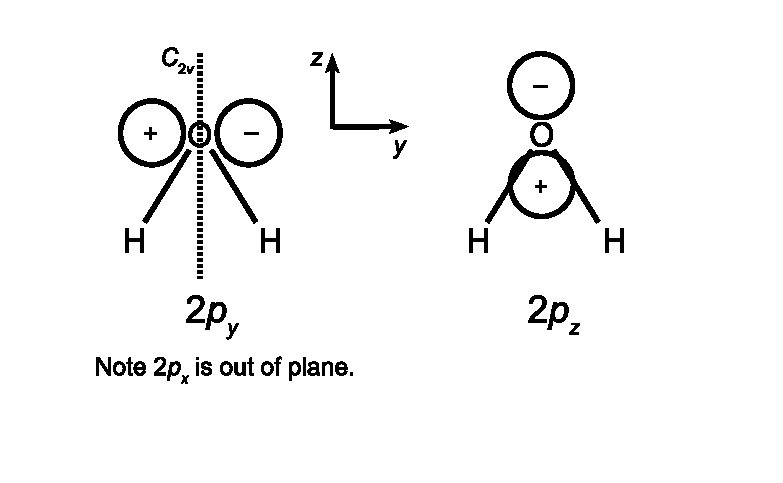
\includegraphics[scale=0.45]{watermo2}
\caption{Visualization of oxygen atom orbitals.}
\end{figure}
The $2s$ O orbital is clearly $A_1$ (totally symmetric). According to the above picture, $2p_z$ is also $A_1$. $p_y$ appears to
be $B_2$ and $p_x$ $B_1$. To find possible non-zero overlap integral value ($S$), we have to find pairs that produce $A_1$ when multiplied. Essentially, this says
that they must have the same symmetry. Thus $S_1$ can combine with $2s$ and $2p_z$ and $S_2$ with $2p_y$.\\

\hrule\vspace{0.5cm}



